\chapter{Sample Imputation via Conditional Generative Adversarial Networks}
\label{chap:SICG}

\section{Introduction}
\label{sec:sicg_intro}

Chapter~\ref{chap:SISL} asked whether the sampling weight of a two-phase design has a role inside the imputation model, and not only inside the analysis model where it is conventionally applied. The answer depends on whether the variables that drove phase-two selection are available to the analyst. When they are available, the imputation can condition on them, so that conditioning already removes the selection effect and the released weight adds little to the imputation model. When they are suppressed, as in the privacy-constrained design of Chapter~\ref{chap:SISL} where the stratifying variables behind $\pi_i$ are withheld, conditioning cannot remove that effect and the weight must carry the correction. That setting is a narrow one, in which the design is driven by withheld variables and only the weight remains in the released file.

The present chapter takes the first of those settings. When the variables that drive phase-two selection are recorded at phase one and the imputation conditions on them, the validated values are selected on observed information, and the inclusion probability is no longer a component of the imputation model but at most a design weight that guards against covariate shift. What then remains is the modelling problem itself: to estimate the conditional distribution $P(X_i\mid\tilde{X}_i,Z_i,A_i,Y_i)$ faithfully and to propagate its uncertainty. Chapter~\ref{chap:ImpReview} reviewed the candidate models, from the chained equations of \texttt{mice} \citep{vanBuuren2011} and the gradient-boosted trees of \texttt{mixgb} \citep{deng2024multiple} to the deep generative architectures GAIN \citep{yoon2018gain} and TabCSDI \citep{zheng2022diffusion}, and concluded that none was designed for the structural constraints of a two-phase validation study. This chapter asks whether a neural generative model can meet those constraints.

Against the tree-based and chained-equation methods, a neural generator offers two practical advantages here. It models the joint conditional distribution $P(X_i\mid\tilde{X}_i,Z_i,A_i,Y_i)$ directly rather than decomposing it into a sequence of univariate conditionals, and it returns mixed continuous and categorical outputs in a single forward pass.

The starting point pursued here does not come from the imputation literature. The deep generative imputation methods reviewed in Chapter~\ref{chap:ImpReview} share an architectural assumption that is poorly matched to two-phase data: they spend capacity learning or adapting to the missingness pattern, which in this setting is known and identical across all unvalidated individuals. GAIN trains a discriminator to classify which entries are observed against imputed \citep{yoon2018gain}, and TabCSDI applies self-supervised random masking to expose the network to many missingness configurations \citep{zheng2022diffusion}. Under a known missing design neither capability is the main requirement, because the missing block is fixed by the phase-two indicator $R_i$ and needs no learning. What is required instead is a model that conditions on a large set of fully observed covariates and generates the missing block, a task closer to conditional tabular generation than to general-purpose imputation. The more appropriate starting point is therefore the tabular data generation literature. \citet{xu2019modeling} proposed the Conditional Tabular GAN (CTGAN) and \citet{zhao2022ctabganplus} the Conditional Tabular GAN+ (CTAB-GAN+); both show that a Wasserstein generative adversarial network with tabular-specific encoding can produce synthetic data of sufficient quality for downstream modelling, although neither reported inferential summaries such as coefficient bias or coverage. This chapter adapts that generation framework to imputation in the two-phase setting.

Sample Imputation via Conditional Generative Adversarial Networks (SICG) differs from both the existing imputation and generation methods in three respects. First, the generator does not synthesise whole rows from noise and does not reconstruct masked entries from partial inputs; it conditions on the observed block $(\tilde{X}_i,C_i)$ and outputs only the missing phase-two block $X_i$, so the task reduces to learning $P(X_i\mid\tilde{X}_i,C_i)$ within an adversarial framework. Second, the critic receives the full completed record, so the adversarial signal reflects the joint plausibility of the imputed values in their covariate context. Third, to address the parameter-uncertainty gap discussed in Chapter~\ref{chap:ImpReview}, between-imputation variability is generated by Monte Carlo dropout on the trained generator, with bootstrap retraining and Stochastic Weight Averaging-Gaussian (SWAG) examined as alternatives \citep{gal2016dropout,maddox2019simple}. The contribution is not a new adversarial architecture but the demonstration that an existing tabular generation framework can be repurposed for two-phase imputation, with an assessment of whether it yields valid inference under the coefficient-bias and coverage criteria the generation literature has not considered. The contents of $C_i$ depend on the study setting and are defined in Section~\ref{sec:sicg_problem}.

Section~\ref{sec:sicg_background} reviews the components of the CTGAN/CTAB-GAN+ framework that SICG inherits. Section~\ref{sec:sicg_method} describes the adaptations for two-phase imputation. Section~\ref{sec:sicg_ablation} reports the staged ablation that fixed each component of the method, with the empirical evidence for every decision. Section~\ref{sec:sicg_sim} then evaluates the retained configuration against the baselines under the framework of Chapter~\ref{chap:SimDesigns}. Section~\ref{sec:sicg_discussion} discusses the findings.


\section{Background}
\label{sec:sicg_background}

The GAN framework and its application to tabular data imputation were introduced in Section~\ref{sec:gans}, which described the minimax objective (equation~\ref{eq:gan_obj}), the Jensen--Shannon divergence under the optimal discriminator, and the GAIN architecture. The present section focuses on the components of the tabular data \emph{generation} literature that SICG inherits, not covered in Chapter~\ref{chap:ImpReview}: the WGAN-GP training objective (Section~\ref{sec:sicg_wgangp}) and the architecture and encoding choices validated by CTGAN and CTAB-GAN+ (Section~\ref{sec:sicg_arch}).


\subsection{The WGAN-GP training objective}
\label{sec:sicg_wgangp}

CTGAN and CTAB-GAN+ train with the Wasserstein objective and gradient penalty (WGAN-GP) rather than the original minimax objective of \citet{goodfellow2014generative}. In the original GAN game, the discriminator separates samples from the data distribution \(P_r\) and the generator distribution \(P_g\), while the generator is trained through the discriminator's response. At the optimal discriminator, this game corresponds to minimising the Jensen--Shannon divergence between \(P_r\) and \(P_g\). If the two distributions are concentrated on separated or nearly separated supports, the discriminator can distinguish them with little ambiguity and the divergence saturates. Small movements of the generator may then produce little change in the objective, leaving a weak or uninformative gradient even when the generated distribution remains far from the data distribution \citep{arjovsky2017principled}.

The Wasserstein-1 distance, stated formally in Appendix~\ref{app:wasserstein}, measures the cost of transporting probability mass from one distribution to the other. When separated distributions move closer, the distance changes with that movement. A Wasserstein generative adversarial network (WGAN) can therefore provide a more informative training signal than the Jensen--Shannon objective when the original GAN loss saturates \citep{arjovsky2017wasserstein}. SICG adopts WGAN-GP because this training objective is used in tabular GAN architectures such as CTGAN and CTAB-GAN+ and is less prone to saturation on separated supports.

Formally, the Wasserstein-1 distance is the smallest average distance the mass of one distribution must be moved to match the other. It cannot be minimised over its defining couplings directly, but its Kantorovich--Rubinstein dual rewrites the same distance as a maximisation over $1$-Lipschitz functions. That dual is the form used in training: a critic network plays the role of the function, returning a real-valued score rather than a probability, and its average score difference between real and generated records estimates the transport cost. Appendix~\ref{app:wasserstein} states the primal distance, the dual, and the Lipschitz constraint that ties them together.

The remaining question is how to impose this Lipschitz restriction in a neural network. \citet{arjovsky2017wasserstein} used weight clipping, but \citet{gulrajani2017improved} showed that clipping can lead to unstable optimisation and poor use of critic capacity. WGAN-GP replaces hard clipping with a soft penalty on the norm of the critic's gradient with respect to its input, evaluated at points interpolated between real and generated samples:
\begin{equation}
\mathcal{L}_D = \mathbb{E}_{z}[D(G(z))] - \mathbb{E}_{x \sim p_{\text{data}}}[D(x)] + \lambda \, \mathbb{E}_{x_{\text{ip}}}[(\|\nabla_{x_{\text{ip}}} D(x_{\text{ip}})\|_2 - 1)^2],
\label{eq:wgan-gp}
\end{equation}
where \(x_{\text{ip}}=\alpha x+(1-\alpha)G(z)\), \(\alpha\sim\mathrm{Uniform}(0,1)\), denotes a random interpolation between a real and a generated sample, and \(\lambda>0\) controls the penalty strength. The penalty encourages the gradient norm to remain close to one on the sampled interpolation points. It is therefore a practical enforcement device for the Wasserstein objective, not a proven mechanism for balancing heterogeneous tabular dimensions. The generator loss is \(\mathcal{L}_G=-\mathbb{E}_z[D(G(z))]\).

Discriminator overfitting under limited training data is also a known difficulty in GAN training and has motivated data-efficient regularisation methods \citep{karras2020training, zhao2020differentiable}. This observation is relevant to the small validated samples used in two-phase studies, but it is not used here as evidence that WGAN-GP solves the limited-data problem. SICG fixes WGAN-GP as part of the inherited CTGAN-style training objective; alternative adversarial losses are not compared in the ablation of Section~\ref{sec:sicg_ablation}. What the simulation study of Section~\ref{sec:sicg_sim} assesses is whether imputations produced under this objective support the target inferential analysis.


\subsection{Architecture and encoding from the generation literature}
\label{sec:sicg_arch}

GANs for tabular data synthesis have been developed through a sequence of methods. \citet{choi2017generating} proposed MedGAN, combining an auto-encoder with a GAN to generate synthetic electronic health records. MedGAN used min-max normalisation to scale continuous variables to $[0,1]$ and could handle either continuous or discrete outputs, but struggled with mixed-type columns and suffered from training instability. \citet{park2018data} proposed TableGAN, which used a convolutional neural network (CNN) generator and discriminator and added an information loss matching first- and second-order discriminator-feature statistics between real and generated batches. TableGAN also added a classifier to penalise semantically inconsistent records. It used min-max normalisation to $[-1,1]$ to match the \texttt{tanh} output activation, which worked for single-mode continuous distributions but could not capture multimodal structure.

\citet{xu2019modeling} proposed CTGAN, which addressed the remaining limitations through three mechanisms. The first is mode-specific normalisation: each continuous value is encoded as a (scalar, one-hot mode indicator) pair using a variational Gaussian mixture model, which allows the generator to represent multimodal distributions that min-max normalisation collapses. The second is a conditional vector with training-by-sampling: the generator receives a mask specifying a particular category of a particular discrete column, and training data are resampled using log-frequency weighting to give minority categories adequate representation. The third is a fully connected residual architecture with WGAN-GP training and PacGAN packing \citep{lin2018pacgan}. PacGAN presents several records jointly to the critic, making a generated distribution with limited sample diversity easier to distinguish from the observed data. The generator recursion is:
\begin{equation}
h_0 = [z,\, c], \qquad h_l = [h_{l-1},\; \text{ReLU}(\text{BN}(W_l h_{l-1} + b_l))], \quad l = 1, \ldots, L,
\label{eq:ctgan-generator}
\end{equation}
where $c$ is the conditioning input, BN denotes batch normalisation and ReLU denotes the rectified linear unit activation. In CTGAN, $c$ is the conditional vector; in SICG it is the observed block $[\tilde{X}_i,C_i]$. Drawing a category is not a differentiable operation, which would block gradient training of the generator; the Gumbel-softmax replaces the hard draw with a differentiable approximation that perturbs the logits with Gumbel noise and applies a temperature-scaled softmax. For categorical logits $\ell_1,\ldots,\ell_K$, the Gumbel-softmax output is
\begin{equation}
y_k=\frac{\exp\{(\ell_k+g_k)/\tau\}}{\sum_{r=1}^K\exp\{(\ell_r+g_r)/\tau\}},
\qquad g_k\stackrel{\mathrm{iid}}{\sim}\mathrm{Gumbel}(0,1),
\label{eq:sicg_gumbel}
\end{equation}
where the temperature $\tau>0$ controls how closely $y$ approaches a one-hot vector. This continuous relaxation permits differentiation through the categorical output during training \citep{jang2017categorical}. At imputation, SICG replaces the relaxation with the category having the largest generator output logit. In their benchmark experiments, CTGAN outperformed prior tabular GANs and Bayesian network baselines on the majority of real datasets under the machine-learning efficacy criterion.

\citet{zhao2022ctabganplus} proposed CTAB-GAN+, building on their earlier CTAB-GAN \citep{zhao2021ctabgan}, which combined architectural elements from prior tabular GANs: the conditional vector and training-by-sampling from CTGAN, the CNN-based generator and information loss from TableGAN, and the WGAN-GP objective. CTAB-GAN+ differs from CTGAN in two structural respects. First, it replaces the fully connected generator and discriminator with CNNs that reshape each tabular row into a square matrix, introducing a spatial adjacency structure into the data representation. Second, it augments the generator loss with two auxiliary terms: the information loss inherited from TableGAN, and a downstream loss from an auxiliary classifier or regressor trained on the real data. They also introduced a mixed-type encoder for variables containing both categorical and continuous values, a general transform for single-Gaussian columns where mode-specific normalisation is unnecessarily complex, and a log-transform for long-tailed distributions. Together these components improved synthetic data utility by at least 41.2\% in accuracy relative to the best prior baseline across five classification datasets. Of the two, only CTGAN reported statistical inference metrics, via likelihood; CTAB-GAN+ evaluated exclusively through machine learning utility and statistical similarity measures.

SICG inherits the generator recursion~\eqref{eq:ctgan-generator}, the WGAN-GP objective~\eqref{eq:wgan-gp}, and the Gumbel-softmax activation. It excludes mode-specific normalisation, category-rebalanced training, the CNN architecture of CTAB-GAN+, and the auxiliary losses. The reasons are evaluated in Section~\ref{sec:sicg_ablation}. The generator is trained on the validated subsample and conditions on the variables observed at phase one. This identifies the target conditional distribution when validation is conditionally independent of the target block and the required covariate profiles have validated support. The deterministic tail designs do not satisfy positivity over the full cohort, so their results also assess extrapolation beyond the validated region.


\section{Method}
\label{sec:sicg_method}

This section describes the adaptations that convert the generation framework of Section~\ref{sec:sicg_background} into an imputation method for two-phase validation studies. Section~\ref{sec:sicg_problem} formulates the imputation task, Section~\ref{sec:sicg_encoding} the data encoding, Section~\ref{sec:sicg_training} the training objective, and Section~\ref{sec:sicg_mi} the procedure for generating multiple completed datasets. The complete method is summarised in Algorithm~\ref{alg:sicg}.


\subsection{Problem formulation}
\label{sec:sicg_problem}

We adopt the notation of Chapter~\ref{chap:background}. Let $X_i$ denote the block whose validated values are observed only when $R_i=1$, let $\tilde X_i$ collect its phase-one proxies, and let $C_i$ collect the remaining variables observed for every cohort member. In the \texttt{SampleE} settings, $C_i=(Z_i,A_i,Y_i)$ and $X_i$ contains the validated covariates. In \texttt{SampleOE}, the validated event time, event indicator and censoring time are also included in $X_i$, while their phase-one proxies remain in the observed block. Thus $X_i$ denotes the complete validation target rather than covariates alone. For the probability sampling designs, $R_i$ has a known inclusion probability; the deterministic tail designs instead have a known selection rule without positive inclusion probability for every unit.

The imputation task is to generate draws from $P(X_i\mid\tilde X_i,C_i)$ for each individual with $R_i=0$. A model fitted on the validated rows targets this conditional distribution when $R_i$ is conditionally independent of $X_i$ given $(\tilde X_i,C_i)$ and the relevant conditioning profiles have validated support. SICG adapts the CTGAN generator~\eqref{eq:ctgan-generator} by replacing the conditional vector with the observed block and restricting the output to $X_i$:
\begin{equation}
\hat{X}_i = G_\theta(z_i, \tilde{X}_i, C_i), \quad z_i \sim \mathcal{N}(0, I_{d_z}).
\label{eq:sicg-generator}
\end{equation}
The critic receives the concatenated record $[\hat{X}_i,\tilde{X}_i,C_i]$ or $[X_i,\tilde{X}_i,C_i]$ and is trained with~\eqref{eq:wgan-gp}. Figure~\ref{fig:sicg-architecture} shows the \texttt{SampleE} form, where the outcome is fully observed; \texttt{SampleOE} moves the validated outcome components into the target block as described above.

\begin{sidewaysfigure}
\centering
\resizebox{0.95\textheight}{!}{%
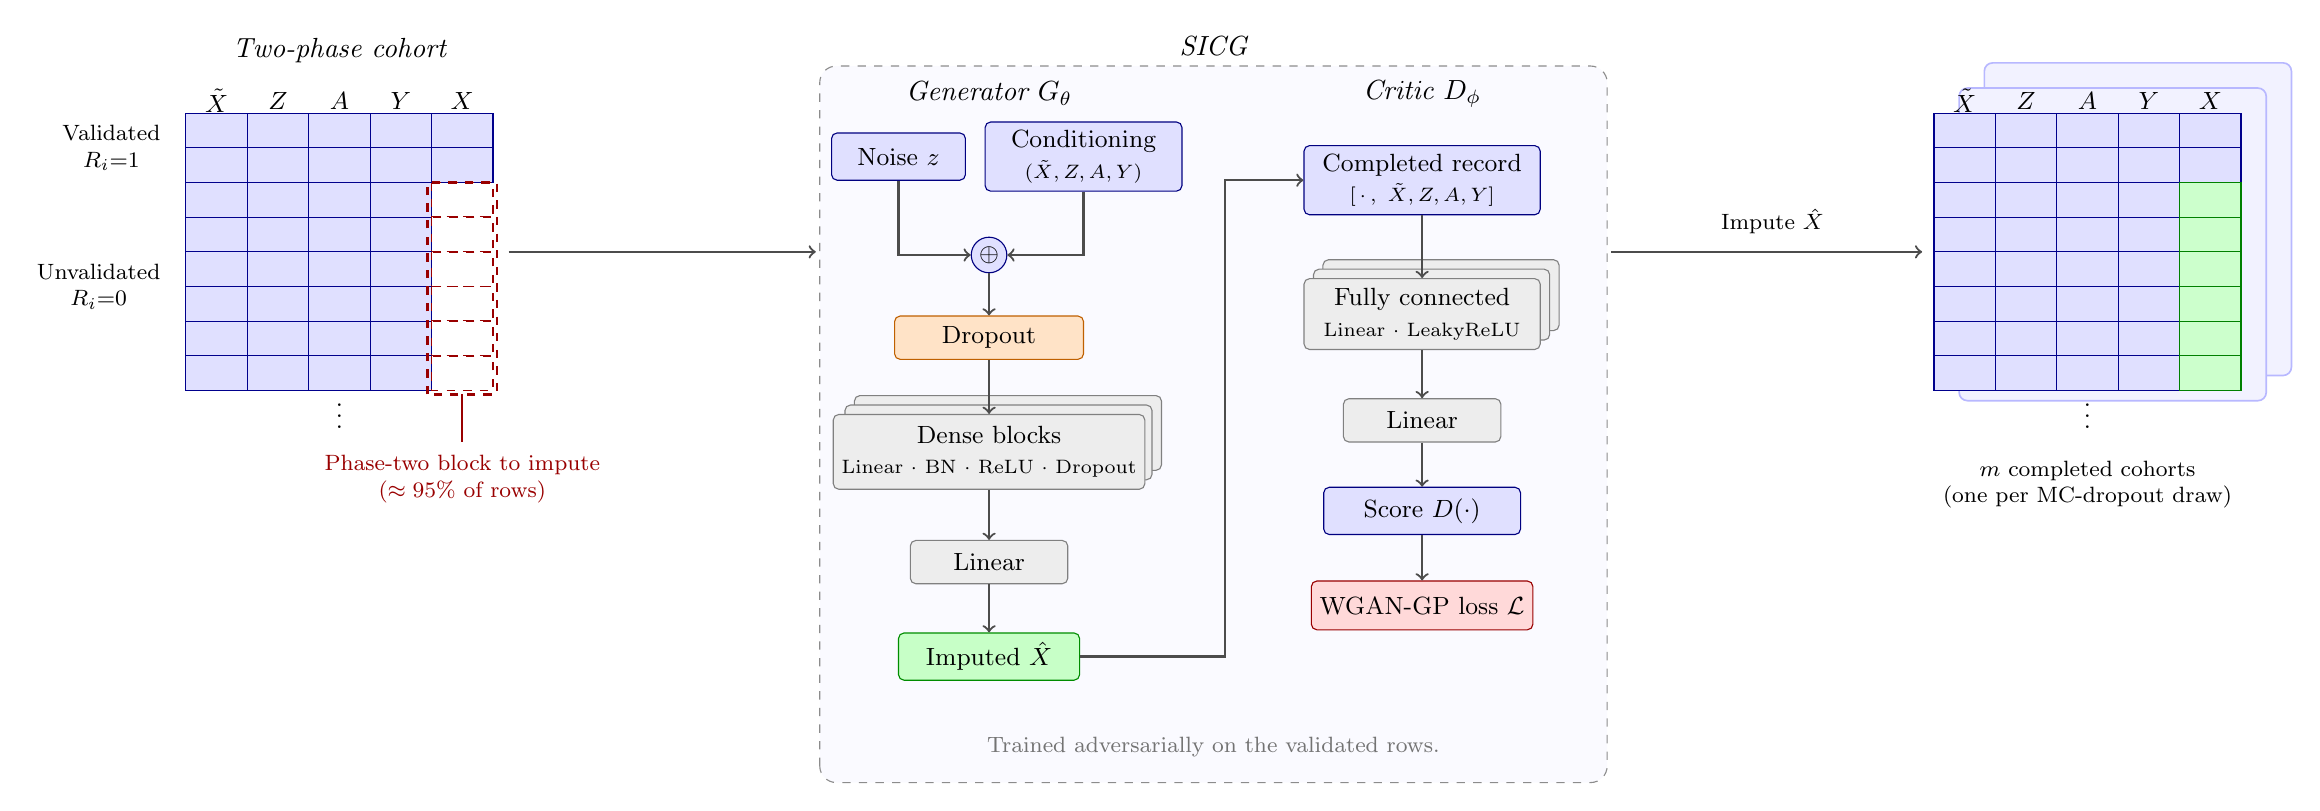
\begin{tikzpicture}[
  every node/.style={font=\small},
  obs/.style={fill=blue!12, draw=blue!55!black, line width=0.4pt},
  mis/.style={fill=white, draw=red!60!black, dashed, line width=0.6pt},
  imp/.style={fill=green!20, draw=green!50!black, line width=0.4pt},
  data/.style={rounded corners=2pt, draw=blue!50!black, fill=blue!12, align=center, inner sep=3pt},
  lyr/.style={rounded corners=2pt, draw=black!50, fill=black!7, align=center, inner sep=3pt},
  drp/.style={rounded corners=2pt, draw=orange!75!black, fill=orange!22, align=center, inner sep=3pt},
  impbox/.style={rounded corners=2pt, draw=green!55!black, fill=green!22, align=center, inner sep=3pt},
  loss/.style={rounded corners=2pt, draw=red!60!black, fill=red!15, align=center, inner sep=3pt},
  cont/.style={rounded corners=6pt, draw=black!45, dashed, fill=blue!2},
  ghost/.style={rounded corners=3pt, fill=blue!5, draw=blue!28, line width=0.6pt},
  arr/.style={->, line width=0.8pt, draw=black!70},
]
% ===== SICG container (behind) =====
\draw[cont] (9.55,3.5) rectangle (19.55,12.6);
% ===== two-phase cohort (left) =====
\begin{scope}[shift={(1.5cm,12.0cm)}, x=0.78cm, y=0.44cm]
  \foreach \x/\lab in {0.5/{$\tilde{X}$}, 1.5/{$Z$}, 2.5/{$A$}, 3.5/{$Y$}, 4.5/{$X$}} \node at (\x,0.36) {\lab};
  \foreach \r in {0,1} \foreach \c in {0,1,2,3,4} \draw[obs] (\c,-\r) rectangle ++(1,-1);
  \foreach \r in {2,3,4,5,6,7} {
    \foreach \c in {0,1,2,3} \draw[obs] (\c,-\r) rectangle ++(1,-1);
    \draw[mis] (4,-\r) rectangle ++(1,-1);
  }
  \node at (2.5,-8.5) {$\vdots$};
\end{scope}
\node[font=\itshape] at (3.45,12.8) {Two-phase cohort};
\node[anchor=east, font=\footnotesize, align=center] at (1.3,11.56) {Validated\\$R_i{=}1$};
\node[anchor=east, font=\footnotesize, align=center] at (1.3,9.8) {Unvalidated\\$R_i{=}0$};
\draw[red!60!black, dashed, line width=0.9pt] (4.57,8.43) rectangle (5.45,11.12);
\draw[red!60!black, line width=0.6pt] (5.01,8.43) -- (5.01,7.82);
\node[anchor=north, font=\footnotesize, text=red!60!black, align=center] at (5.01,7.78) {Phase-two block to impute\\($\approx 95\%$ of rows)};
% ===== SICG internals (centre) =====
\node[font=\itshape] at (14.55,12.85) {SICG};
\node[font=\itshape] at (11.7,12.25) {Generator $G_\theta$};
\node[font=\itshape] at (17.2,12.25) {Critic $D_\phi$};
% generator
\node[data, minimum width=1.7cm, minimum height=0.6cm] (z) at (10.55,11.45) {Noise $z$};
\node[data, minimum width=2.5cm, minimum height=0.78cm] (co) at (12.9,11.45) {Conditioning\\{\scriptsize $(\tilde{X}, Z, A, Y)$}};
\node[circle, draw=blue!50!black, fill=blue!12, inner sep=1.2pt] (cat) at (11.7,10.2) {$\oplus$};
\node[drp, minimum width=2.4cm, minimum height=0.55cm] (dp) at (11.7,9.15) {Dropout};
\draw[lyr] (9.99,7.465) rectangle ++(3.9,0.95);
\draw[lyr] (9.87,7.345) rectangle ++(3.9,0.95);
\node[lyr, minimum width=3.9cm, minimum height=0.95cm] (dn) at (11.7,7.7) {Dense blocks\\{\scriptsize Linear $\cdot$ BN $\cdot$ ReLU $\cdot$ Dropout}};
\node[lyr, minimum width=2.0cm, minimum height=0.55cm] (ln) at (11.7,6.3) {Linear};
\node[impbox, minimum width=2.3cm, minimum height=0.6cm] (xh) at (11.7,5.1) {Imputed $\hat{X}$};
\draw[arr] (z.south) -- (10.55,10.2) -- (cat.west);
\draw[arr] (co.south) -- (12.9,10.2) -- (cat.east);
\draw[arr] (cat.south) -- (dp.north);
\draw[arr] (dp.south) -- (dn.north);
\draw[arr] (dn.south) -- (ln.north);
\draw[arr] (ln.south) -- (xh.north);
% critic
\node[data, minimum width=3.0cm, minimum height=0.82cm] (rec) at (17.2,11.15) {Completed record\\{\scriptsize $[\,\cdot\,,\ \tilde{X}, Z, A, Y]$}};
\draw[lyr] (15.94,9.24) rectangle ++(3.0,0.9);
\draw[lyr] (15.82,9.12) rectangle ++(3.0,0.9);
\node[lyr, minimum width=3.0cm, minimum height=0.9cm] (fcb) at (17.2,9.45) {Fully connected\\{\scriptsize Linear $\cdot$ LeakyReLU}};
\node[lyr, minimum width=2.0cm, minimum height=0.55cm] (ln2) at (17.2,8.1) {Linear};
\node[data, minimum width=2.5cm, minimum height=0.6cm] (sc) at (17.2,6.95) {Score $D(\cdot)$};
\node[loss, minimum width=2.8cm, minimum height=0.62cm] (ls) at (17.2,5.75) {WGAN-GP loss $\mathcal{L}$};
\draw[arr] (rec.south) -- (fcb.north);
\draw[arr] (fcb.south) -- (ln2.north);
\draw[arr] (ln2.south) -- (sc.north);
\draw[arr] (sc.south) -- (ls.north);
% adversarial feed
\draw[arr] (xh.east) -- (14.7,5.1) -- (14.7,11.15) -- (rec.west);
\node[font=\footnotesize, text=black!55] at (14.55,3.95) {Trained adversarially on the validated rows.};
% cohort -> SICG
\draw[arr] (5.6,10.24) -- (9.5,10.24);
% ===== m completed cohorts (right) =====
\draw[ghost] (24.34,8.67) rectangle ++(3.9,3.97);
\draw[ghost] (24.02,8.35) rectangle ++(3.9,3.97);
\begin{scope}[shift={(23.7cm,12.0cm)}, x=0.78cm, y=0.44cm]
  \foreach \x/\lab in {0.5/{$\tilde{X}$}, 1.5/{$Z$}, 2.5/{$A$}, 3.5/{$Y$}, 4.5/{$X$}} \node at (\x,0.36) {\lab};
  \foreach \r in {0,1} \foreach \c in {0,1,2,3,4} \draw[obs] (\c,-\r) rectangle ++(1,-1);
  \foreach \r in {2,3,4,5,6,7} {
    \foreach \c in {0,1,2,3} \draw[obs] (\c,-\r) rectangle ++(1,-1);
    \draw[imp] (4,-\r) rectangle ++(1,-1);
  }
  \node at (2.5,-8.5) {$\vdots$};
\end{scope}
\node[anchor=north, font=\footnotesize, align=center] at (25.65,7.71) {$m$ completed cohorts\\(one per MC-dropout draw)};
\draw[arr] (19.6,10.24) -- (23.55,10.24);
\node[font=\footnotesize, anchor=south] at (21.65,10.34) {Impute $\hat{X}$};
\end{tikzpicture}%
}
\caption{SICG in the \texttt{SampleE} setting. The validated target block $X$ is observed when $R_i=1$ and imputed otherwise. The generator takes noise and the observed block $(\tilde X,Z,A,Y)$ and outputs $\hat X$. The critic compares completed and validated records under the gradient-penalised Wasserstein objective. With dropout active at prediction, $m$ generator runs produce $m$ completed cohorts whose analysis estimates are combined by Rubin's rules. In \texttt{SampleOE}, validated outcome components are included in the target block and their proxies remain observed.}
\label{fig:sicg-architecture}
\end{sidewaysfigure}


\subsection{Data encoding}
\label{sec:sicg_encoding}

The phase-two targets $X_i$ mix continuous clinical measurements with categorical diagnostic variables, encoded separately. Each continuous variable is standardised by the $z$-score computed on the validated subsample $\{i : R_i = 1\}$, preceded, for the severely right-skewed variables, by a $\log(1 + x + s)$ shift in which $s$ is the smallest constant making the argument positive. Each categorical variable is one-hot encoded, with any missing level inside the phase-two block treated as an additional category; the generator emits one logit per level, passed through the Gumbel-softmax reparameterisation \citep{jang2017categorical} during training and replaced by a hard $\arg\max$ at imputation time. Phase-one variables $\tilde{X}_i$ and conditioning covariates $C_i$ use the same $z$-score and one-hot encodings, but with parameters from the full cohort, since they are observed for every individual.

After encoding, the generator output is partitioned by a fixed layout that routes the identity activation, clamped to $[-5, 5]$, to the continuous dimensions and the Gumbel-softmax to each categorical block.


\subsection{Training objective}
\label{sec:sicg_training}

The training objective follows the WGAN-GP framework of Section~\ref{sec:sicg_wgangp}. At each step the critic is updated $n_D$ times and the generator once. The critic loss is:
\begin{equation}
\mathcal{L}_D = \frac{1}{B}\sum_{i=1}^B D(\hat{X}_i, \tilde{X}_i, C_i) - \frac{1}{B}\sum_{i=1}^B D(X_i, \tilde{X}_i, C_i) + \lambda_{\text{GP}} \cdot \text{GP}(D),
\label{eq:sicg-d-loss}
\end{equation}
where $\text{GP}(D)$ is the gradient penalty term computed on interpolations between real and fake records, as defined in Section~\ref{sec:sicg_wgangp}, and $\lambda_{\text{GP}}$ controls its weight. The generator loss consists of the adversarial term alone:
\begin{equation}
\mathcal{L}_G = -\frac{1}{B}\sum_{i=1}^B D(G_\theta(z_i, \tilde{X}_i, C_i), \tilde{X}_i, C_i).
\label{eq:sicg-g-loss}
\end{equation}

No reconstruction loss, such as squared error between $\hat{X}_i$ and the observed $X_i$, is included in the generator objective. A squared-error term pulls the generated values toward the conditional mean and can reduce their spread. Lemma~\ref{lemma:mean-collapse} formalises the limiting case: as the reconstruction penalty dominates the remaining objective, the generator concentrates on the conditional mean and the resulting between-imputation variance tends to zero. The lemma does not establish collapse for every finite penalty. The finite comparison in Section~\ref{sec:sicg_ablation} instead shows what occurred in the tested SICG setting: adding the reconstruction term reduced the marginal standard deviation of the imputed values by $9.5\%$ and the between-imputation variance of the fitted coefficient by $72\%$. Since about $95\%$ of the phase-two block is imputed in these simulations, this reduction in between-imputation variation can materially reduce Rubin's total variance estimate.


\subsection{Generating multiple imputations}
\label{sec:sicg_mi}

Section~\ref{sec:uncertainty_gap} established that a GAN which fixes its parameters $\theta$ after training and varies only the noise input $z_i$ captures data noise but not parameter uncertainty, producing a between-imputation variance $\hat{V}_{\text{between}}$ that is too small for Rubin's combining rules. How to introduce parameter-uncertainty variation into a trained generator is therefore a central design issue for GAN-based multiple imputation. The present study investigated three approaches; each generates between-imputation variability through a different mechanism and carries its own computational cost and theoretical assumptions.

\paragraph{MC-dropout (default).} The first approach, the default in SICG, exploits the dropout layers already present in the generator. \citet{gal2016dropout} showed that a network with dropout before every weight layer can be interpreted as approximate variational inference over the network weights, with the dropout distribution serving as the variational posterior. Under this interpretation, $m$ stochastic forward passes through the trained generator with dropout active at imputation time produce $m$ samples from an approximate posterior predictive distribution. In SICG a single generator is trained once on the full validated subsample. At imputation time the dropout layers remain active while all other layers are fixed, and each of the $m$ passes uses a fresh noise vector $z_i^{(j)} \sim \mathcal{N}(0, I_{d_z})$ and a fresh dropout mask, yielding a different imputed value $\hat{X}_i^{(j)}$.

Computationally this approach is considerably cheaper than the alternatives. Only one generator is trained, and the $m$ imputation passes are forward evaluations with no gradient computation, so the total training cost is $\mathcal{O}(T)$ rather than $\mathcal{O}(m \cdot T)$. MC-dropout has a Bayesian interpretation as an approximate variational predictive procedure \citep{gal2016dropout}, but this interpretation does not guarantee calibrated between-imputation variability. The uncertainty induced by dropout depends on the dropout rate, regularisation scale, architecture and training objective. SICG uses it to vary the imputations and evaluates the resulting interval coverage in Section~\ref{sec:sicg_sim}.

\paragraph{Bootstrap retraining.} The second approach trains $m$ separate generators, each on an independent bootstrap resample of the validated subsample $\{i : R_i = 1\}$. For the $j$-th imputation, a bootstrap sample $\mathcal{B}^{(j)}$ of size $n$ is drawn with replacement, and a fresh generator--critic pair $(G_\theta^{(j)}, D_\phi^{(j)})$ is trained from random initialisation on $\mathcal{B}^{(j)}$. The resamples and refits vary the fitted generator across imputations without positing a parametric distribution over its weights. Bootstrap refitting is also used by \texttt{mice.impute.rf}, while \texttt{mice.impute.cart} uses a Bayesian bootstrap \citep{doove2014recursive,burgette2010multiple}. The current \texttt{mixgb} implementation uses internal XGBoost row subsampling rather than an outer bootstrap and does not use predictive mean matching by default \citep{deng2024multiple}. For SICG, the disadvantage is computational: producing $m$ completed datasets requires $m$ adversarial training runs for every simulation replicate.

\paragraph{SWAG.} The third approach uses Stochastic Weight Averaging-Gaussian (SWAG) \citep{maddox2019simple}, which constructs a Gaussian approximation to the posterior over the generator weights from snapshots of the weight trajectory during training. A single generator is trained using stochastic gradient descent with a cosine-annealed learning rate schedule, and weight snapshots are collected at regular intervals during the second half of training. Their first and second moments, with a low-rank approximation to their covariance, define a Gaussian $\mathcal{N}(\bar{\theta}, \Sigma_{\text{diag}} + \Sigma_{\text{low-rank}})$ from which generator weights can be sampled at imputation time. Each sampled weight vector $\theta^{(j)}$ yields a different generator, and hence different imputations. Like MC-dropout, SWAG requires only a single training run; unlike MC-dropout, it samples weights from an estimated local Gaussian distribution instead of applying stochastic dropout masks. It assumes that the posterior over $\theta$ is adequately represented by that Gaussian approximation, which may not hold for the highly non-convex loss surfaces of adversarial training. The method is also usually paired with SGD rather than Adam, because its approximation is built from the SGD weight trajectory considered by \citet{maddox2019simple}. For an adversarial generator this is a practical disadvantage: the GAN literature commonly uses adaptive optimisers to stabilise the minimax training dynamics, and plain SGD is more prone to oscillation in such games \citep{mescheder2018which, salimans2016improved}.

\paragraph{Summary.} MC-dropout requires one generator fit, bootstrap retraining requires $m$ fits, and SWAG requires one fit with the optimiser and weight-sampling procedure described above. All three use the same generator architecture, training objective and data encoding. They differ in how they vary the fitted network or its output across completed datasets. Section~\ref{sec:sicg_sim} compares the resulting interval coverage.

The complete procedure under the default MC-dropout configuration is summarised in Algorithm~\ref{alg:sicg}.

\begin{algorithm}[t]
\caption{Sample imputation via conditional generative adversarial networks (SICG)}
\label{alg:sicg}
\begin{algorithmic}[1]
\Require Observed block $\{(\tilde{X}_i,C_i) : i = 1, \ldots, N\}$; validated targets $\{X_i : R_i = 1\}$; number of imputations $m$; training steps $T$; critic steps $n_D$; noise dimension $d_z$; gradient penalty weight $\lambda_{\text{GP}}$; Gumbel temperature $\tau$; dropout rate $\rho$
\Statex
\State Encode all variables (Section~\ref{sec:sicg_encoding}); compute layout $\mathcal{L}$
\State Initialise generator $G_\theta$ and critic $D_\phi$
\For{$t = 1, \ldots, T$} \Comment{Training (single fit)}
    \For{$d = 1, \ldots, n_D$}
        \State Sample mini-batch $\{i_1, \ldots, i_B\}$ from $\{i : R_i = 1\}$
        \State $z_i \sim \mathcal{N}(0, I_{d_z})$ for each $i$ in the mini-batch
        \State $\hat{X}_i \gets \text{GumbelActivate}(G_\theta(z_i, \tilde{X}_i, C_i), \mathcal{L}, \tau)$
        \State Update $D_\phi$ by descending $\nabla_\phi \mathcal{L}_D$ \hfill (equation~\ref{eq:sicg-d-loss})
    \EndFor
    \State Sample mini-batch from $\{i : R_i = 1\}$; generate $z_i \sim \mathcal{N}(0, I_{d_z})$
    \State $\hat{X}_i \gets \text{GumbelActivate}(G_\theta(z_i, \tilde{X}_i, C_i), \mathcal{L}, \tau)$
    \State Update $G_\theta$ by descending $\nabla_\theta \mathcal{L}_G$ \hfill (equation~\ref{eq:sicg-g-loss})
\EndFor
\Statex
\For{$j = 1, \ldots, m$} \Comment{Imputation with MC-dropout}
    \State Activate dropout layers in $G_\theta$ (rate $\rho$); fix all other layers
    \For{each $i$ with $R_i = 0$}
        \State $z_i^{(j)} \sim \mathcal{N}(0, I_{d_z})$
        \State $\hat{X}_i^{(j)} \gets \text{HardActivate}(G_\theta(z_i^{(j)}, \tilde{X}_i, C_i), \mathcal{L})$ \quad \emph{(dropout mask active)}
        \State Inverse-transform $\hat{X}_i^{(j)}$ to original scale
    \EndFor
\EndFor
\Ensure $m$ completed datasets $\{\hat{X}_i^{(j)} : R_i = 0,\; j = 1, \ldots, m\}$
\end{algorithmic}
\end{algorithm}


\section{Ablation Study}
\label{sec:sicg_ablation}

The configuration of SICG was settled by a staged ablation rather than a single head-to-head comparison. Starting from the plain WGAN-GP conditional generator, the ablation tests additional components drawn from GAN training practice, tabular generation models and multiple-imputation uncertainty mechanisms. The retention criterion is inferential: a component is retained only when it improves the downstream Cox-model estimates after imputation, with particular attention to bias, nominal coverage and the oracle coverage diagnostics. A generator can fit the observed phase-two block closely and may nevertheless return confidence intervals that are too narrow, so pointwise reconstruction accuracy is not sufficient for the decisions made in this section.

Table~\ref{tab:sicg_ablation} reports the ablation columns in the order in which they are discussed. The first block compares the plain WGAN-GP generator with three additions taken from tabular GAN training: packing (PACK), the discriminator-feature information loss (INFO), and moment matching on a decorrelated projection (MML). The second block tests losses or targets that use observed phase-one information more directly: categorical cross-entropy (CE), a semi-supervised reconstruction task on unvalidated rows (SEMI), and residual generation around the phase-one proxy (RES). The final block compares three ways of producing variation across the \(m\) completed datasets: bootstrap retraining (BOOT), SWAG, and MC-dropout (DROP).

\subsection{Setup}
\label{sec:sicg_ablation_setup}

The ablation uses the \texttt{SampleE} version of Simulation Design~III under \texttt{SRS}, as defined in Section~\ref{sec:sim2context} and specified in Appendix~\ref{app:sim2}. This setting isolates imputation of the phase-two covariate block: the survival outcome is observed, while the validated covariates are available only for the phase-two subsample. Each replicate has \(N=20{,}000\), \(n=1{,}000\), and \(m=5\) completed datasets. Results are summarised by coefficient blocks rather than by individual coefficient, following the main simulation tables.

\subsection{Generator and adversarial loss}
\label{sec:sicg_ablation_generator}

The first stage fixed the backbone. Four candidates were compared: the unpacked WGAN-GP generator of Section~\ref{sec:sicg_arch}; the same generator with PacGAN packing \citep{lin2018pacgan}, as used in CTGAN \citep{xu2019modeling}; the unpacked generator with the information loss of TableGAN \citep{park2018data}, which matches critic-feature statistics for real and generated records and is also used by CTAB-GAN+ \citep{zhao2022ctabganplus}; and a packed generator with a moment-matching penalty on a principal-component projection, following MargCTGAN \citep{afonja2023margctgan}. The auxiliary losses extend the feature-matching idea of \citet{salimans2016improved} to means and covariances \citep{mroueh2017mcgan}. Their source studies assessed distributional similarity and prediction. The present ablation assesses coefficient bias and coverage after imputation.

PACK, INFO and MML change the continuous-block coefficient-estimate summaries only modestly, and nominal coverage remains far below the target for all four single-fit candidates. Their empirical-standard-error oracle coverage is much higher, which indicates that the reported standard errors are small relative to the empirical spread. Packing, information loss and moment matching add complexity without improving the Cox-model quantities used for retention, so the plain unpacked WGAN-GP generator was retained.

\subsection{Reconstruction and structural refinements}
\label{sec:sicg_ablation_refine}

The retained generator carries no reconstruction term. Section~\ref{sec:sicg_training} gives the limiting result for a dominant squared-error penalty; the following comparison records the finite effect in the tested setting.

Simulation Design~II permits a direct check because its analysis has one imputed exposure. Under \texttt{SRS}, the unpacked generator was fitted with and without a squared-error term on the continuous output. Over ten replicates, Table~\ref{tab:sicg_mse} records the standard deviation of the imputed exposure and the between-imputation variance $B$ of its Gaussian-model coefficient. The reconstruction term reduced the first quantity by $9.5\%$ and the second by $72\%$. The direction agrees with the conditional-mean pull in Lemma~\ref{lemma:mean-collapse}, while the observed magnitudes are empirical results for this configuration. Because $B$ measures variation among the completed-data estimates, reducing it lowers the between-imputation part of Rubin's variance. No reconstruction term is retained.

\begin{table}[!htbp]
\centering
\caption{Effect of a squared-error reconstruction loss on the SICG imputations, on Simulation Design~II
  under \texttt{SRS} ($n = 500$ validated, $m = 5$), reported as the mean over ten
  replicates for the single imputed exposure. \emph{SD of imputed values} is the
  standard deviation of the imputed values on the unvalidated rows. \emph{Between-imputation
  variance} $B = (m-1)^{-1}\sum_{k}(\hat\beta_k - \bar\beta)^2$ is the variation among the
  completed-data estimates of the imputed-exposure coefficient in the Gaussian model. The
  reconstruction condition adds a unit-weight squared-error term to the generator loss.}
\label{tab:sicg_mse}
\small
\setlength{\tabcolsep}{8pt}
\begin{tabular}{lrrr}
\toprule
Quantity & No reconstruction & ${}+{}$ reconstruction & Change \\
\midrule
SD of imputed values         & 0.356   & 0.322   & $-9.5\%$ \\
Between-imputation variance   & 0.00494 & 0.00137 & $-72\%$  \\
\bottomrule
\end{tabular}
\end{table}

The next block tested three ways of using observed values more directly. A cross-entropy term on the categorical outputs (the \texttt{loss\_ce} component) was added first, to check whether an explicit supervised loss could improve the categorical part of the imputed block. On the Binary \& Categorical Phase-Two Covariates, the mean bias changed only from \(3.3\%\) to \(3.5\%\), and nominal coverage changed from \(0.745\) to \(0.759\). These changes are too small to justify retaining the term. The cross-entropy loss is therefore treated as an accuracy-oriented categorical penalty that did not materially improve the downstream Cox-model summaries in this ablation.

The semi-supervised variant tested a different idea: whether the \(N-n\) unvalidated records could help the generator through an auxiliary reconstruction task on their phase-one block. In this implementation, those rows do not carry validated \(X_i\), so they cannot enter the critic as real completed examples for the phase-two block. Their contribution is confined to the auxiliary reconstruction loss on variables that are already observed. The table gives no evidence that this extra task improves the Cox summaries enough to retain it. This statement is limited to the SICG implementation tested here.

Residual modelling was motivated by the geometry of the continuous outputs. Generative adversarial networks can be unstable on multimodal continuous columns, and the standard tabular-GAN remedy is the variational Gaussian-mixture normalisation of CTGAN \citep{xu2019modeling}, which encodes each continuous value as a scalar together with a mode indicator. In an imputation task this remedy adds another discrete target to be imputed. SICG therefore tested a simpler alternative: generate the residual \(X_i-\tilde X_i\) around the phase-one proxy instead of generating \(X_i\) directly. This change helped the coefficient-estimate summaries. On the Continuous Phase-Two Covariates, residual modelling gave the lowest mean bias, \(0.2\%\), and the lowest relative RMSE of the coefficient estimate, \(4.9\%\), among the single-fit configurations. It was not retained because the nominal coverage of the same block fell to \(0.299\), below the \(0.374\) of the plain generator. The residual target appears to make the numeric prediction easier to centre, but in this ablation the gain in bias and RMSE is accompanied by a substantial loss of nominal coverage. Across the three blocks, the retained plain generator gives the more acceptable balance for the next stage, where the uncertainty-injection mechanisms are tested directly.

\subsection{Uncertainty injection}
\label{sec:sicg_ablation_uncertainty}

The fourth stage compared bootstrap retraining, MC-dropout and SWAG. Bootstrap retraining varies the fitted generator through a new resample and WGAN-GP fit for each completed dataset. Repeating that adversarial training \(m\) times for every simulation replicate was too costly for the full study. MC-dropout instead trains one generator and retains stochastic dropout masks at imputation. The ablation assesses whether this lower-cost procedure gives tolerable inference for the selected Cox target.

On the continuous phase-two block of the Cox ablation, MC-dropout raises nominal coverage from \(0.374\) under the single-fit generator to \(0.822\), with mean bias \(-0.1\%\) and relative RMSE of \(3.0\%\). Bootstrap gives coverage of \(0.706\) and mean bias of \(3.2\%\) on the same block. This local result supports retaining MC-dropout for SICG, while the comparisons below show that it is not generally the better calibrated uncertainty procedure.

On the categorical block, the bootstrap gives higher nominal coverage than MC-dropout, \(0.942\) against \(0.879\), although MC-dropout has the smaller RMSE. MC-dropout gives zero nominal coverage on the age-by-insulin interaction; bootstrap and SWAG also remain below nominal at \(0.572\) and \(0.500\). Several imputation methods have difficulty with this product term in the full comparison, while raking remains close to nominal coverage. The ablation therefore records a limitation shared across the tested imputation procedures and does not isolate MC-dropout as its cause. These ablation coverages are computed at $m = 5$, whereas the deployed configuration and the Simulation Design~III results in Section~\ref{sec:sicg_sim_surv} use $m = 20$, so the two are not directly comparable. At the smaller $m$ the pooled intervals are wider and the nominal coverage higher; at $m = 20$ they tighten and the coverage falls to the value reported there, exposing the under-propagation of fitted-model variance that this chapter examines.

Table~\ref{tab:sicg_bm} checks how far the Cox ablation can be generalised. For each outcome model, the table reports the between-imputation variance of the fitted analysis coefficient,
\(B=(m-1)^{-1}\sum_{j=1}^m(\hat\beta^{(j)}-\bar\beta)^2\),
after the completed datasets are passed through the analysis model. Each entry is the median \(B\) under the mechanism divided by the median \(B\) under the corresponding single-fit generator. The ratios are therefore scale diagnostics for variance injection. They are not calibrated targets for nominal coverage.

\begin{table}[!htbp]
\centering
\caption{Between-imputation variance \(B\) of the fitted analysis coefficient under each uncertainty mechanism, reported as a median multiple of the corresponding single-fit generator. The Gaussian and Binomial rows refer to Simulation Design~II and pool the two fitted coefficients within each replicate. Their available records comprise 16 single-fit, 10 bootstrap, 15 MC-dropout and 10 SWAG replicates. The Cox row refers to Simulation Design~III and pools five continuous-block coefficients over 500 replicates for each mechanism. Single fit \(\equiv 1\). The ratios compare variance injection with the single-fit baseline; they are not targets for nominal coverage.}
\label{tab:sicg_bm}
\begin{tabular}{lrrr}
\toprule
Outcome model & Bootstrap & MC-dropout & SWAG \\
\midrule
Gaussian, Simulation Design~II & 1540 & 14 & 5 \\
Binomial, Simulation Design~II & 1290 & 42 & 10 \\
Cox, Simulation Design~III & 96 & 28 & 7 \\
\bottomrule
\end{tabular}
\end{table}

The amount of \(B\) produced by MC-dropout differs across the three analysis settings. In the Cox-model setting, MC-dropout gives about \(28\) times the single-fit \(B\), compared with about \(96\) times for bootstrap. In Simulation Design~II, the corresponding comparisons are about \(14\) against \(1540\) in the Gaussian model and \(42\) against \(1290\) in the Binomial model. The settings differ in outcome model, coefficient scale, validation-sample size and the role of the imputed variables in the analysis, so only the ordering within each row can be compared. The Cox ablation supports MC-dropout for that analysis. In Simulation Design~II, the tested MC-dropout procedure produced much less between-imputation variance than bootstrap retraining.

SWAG is not retained because it gives no compensating inferential or computational advantage in this ablation. On the continuous Cox block it has the highest mean bias among the three uncertainty mechanisms, \(5.1\%\), the weakest nominal coverage, \(0.397\), and poorer RMSE than MC-dropout. Its median \(B\) is also smaller than that of MC-dropout in Table~\ref{tab:sicg_bm}. In addition, as discussed in Section~\ref{sec:sicg_mi}, SWAG requires the adversarial generator to be trained with SGD rather than Adam, which made the SICG training less stable and more expensive in the present implementation. These results are sufficient to discard SWAG here, without making a broader claim about SWAG as a method.

The bootstrap injects substantially more between-imputation variance, but its \(m\)-fold WGAN-GP training cost is infeasible at the scale of this simulation study. Among the mechanisms that avoid \(m\) adversarial retrainings, MC-dropout gives the best results on the Cox continuous-covariate ablation target and has the lower computational cost. In Simulation Design~II, it still produces much less between-imputation variance of the fitted coefficient than the bootstrap. The retained SICG configuration is a computational compromise for this study and does not resolve the parameter-uncertainty gap in general.

\begin{landscape}
\begin{table}[!htbp]
\centering
\definecolor{rankone}{RGB}{33,113,181}
\definecolor{ranktwo}{RGB}{107,174,214}
\definecolor{rankthree}{RGB}{198,219,239}
\captionsetup{font=scriptsize}
\caption{Staged ablation for SICG on Simulation Design~III ($N = 20{,}000$, $n = 1{,}000$,
  \texttt{SRS}, $m = 5$, $500$ replicates). The model coefficients are bound into
  blocks: the Continuous Phase-Two Covariates (HbA1c, eGFR, body mass index, insulin), the
  Binary \& Categorical Phase-Two Covariates (the \texttt{rs4506565} genotype and smoking),
  and the age-by-insulin interaction, the single term involving a product of an imputed
  variable. Each entry is the mean of the per-covariate metric across the block; \emph{Rel.\
  RMSE (\%)} is each coefficient's RMSE as a percentage of its true hazard ratio, averaged over
  the block. The reported metrics, Nom.\ Cov., Orc.\ Cov.\ (Emp) and Orc.\ Cov.\ (BC), are defined in
  Section~\ref{sec:eval_metrics}. Columns: complete case (CC), naive
  proxy (UNVAL), unpacked WGAN-GP (UNPK), PacGAN-packed (PACK), ${}+{}$information loss (INFO),
  packed ${}+{}$moment matching (MML), ${}+{}$cross-entropy (CE), ${}+{}$semi-supervised (SEMI),
  ${}+{}$residual modelling (RES), ${}+{}$bootstrap MI (BOOT), ${}+{}$SWAG, and ${}+{}$MC-dropout
  (DROP, retained). The three best distinct ranks among the non-CC/UNVAL methods are shaded;
  displayed ties receive the same shade. VAL is
  omitted, as it defines the truth. The final two blocks report the fully observed
  adjustment covariates, recovered without measurement error for the whole cohort.}
\label{tab:sicg_ablation}
\scriptsize
\setlength{\tabcolsep}{3.5pt}
\adjustbox{max width=\linewidth}{%
\begin{tabular}{lrrrrrrrrrrrr}
\toprule
 & \multicolumn{1}{c}{CC} & \multicolumn{1}{c}{UNVAL} & \multicolumn{1}{c}{UNPK} & \multicolumn{1}{c}{PACK} & \multicolumn{1}{c}{INFO} & \multicolumn{1}{c}{MML} & \multicolumn{1}{c}{CE} & \multicolumn{1}{c}{SEMI} & \multicolumn{1}{c}{RES} & \multicolumn{1}{c}{BOOT} & \multicolumn{1}{c}{SWAG} & \multicolumn{1}{c}{\textbf{DROP}} \\
\midrule
\multicolumn{13}{l}{\textit{Continuous Phase-Two Covariates}} \\[2pt]
\quad Mean Bias (\%) & 0.3 & -0.3 & 2.9 & 1.1 & 3.4 & \cellcolor{rankthree}1.0 & 3.6 & 1.2 & \cellcolor{ranktwo}0.2 & 3.2 & 5.1 & \cellcolor{rankone}-0.1 \\
\quad Rel.\ RMSE (\%) & 5.2 & 8.0 & 7.1 & 6.8 & 7.3 & 7.7 & 7.5 & \cellcolor{rankthree}6.3 & \cellcolor{ranktwo}4.9 & 7.3 & 8.8 & \cellcolor{rankone}3.0 \\
\quad Nom.\ Cov. & 0.945 & 0.153 & 0.374 & 0.358 & 0.365 & 0.337 & 0.370 & 0.372 & 0.299 & \cellcolor{ranktwo}0.706 & \cellcolor{rankthree}0.397 & \cellcolor{rankone}0.822 \\
\quad Orc.\ Cov.\ (Emp) & 0.946 & 0.170 & 0.706 & 0.697 & \cellcolor{ranktwo}0.736 & 0.708 & 0.700 & 0.710 & 0.605 & \cellcolor{rankthree}0.714 & 0.665 & \cellcolor{rankone}0.912 \\
\quad Orc.\ Cov.\ (BC) & 0.948 & 0.913 & 0.537 & 0.518 & 0.501 & 0.470 & 0.522 & 0.512 & 0.617 & \cellcolor{rankone}0.854 & \cellcolor{rankthree}0.623 & \cellcolor{ranktwo}0.834 \\
\midrule
\multicolumn{13}{l}{\textit{Binary \& Categorical Phase-Two Covariates}} \\[2pt]
\quad Mean Bias (\%) & 4.9 & 6.3 & 3.3 & 4.9 & \cellcolor{ranktwo}3.0 & 6.0 & 3.5 & \cellcolor{rankthree}3.2 & 6.0 & 4.3 & \cellcolor{rankone}1.6 & 4.0 \\
\quad Rel.\ RMSE (\%) & 32.8 & 11.6 & 15.9 & \cellcolor{rankthree}13.4 & 15.2 & 15.9 & 16.3 & \cellcolor{ranktwo}12.1 & 16.9 & 15.2 & \cellcolor{rankone}9.6 & 14.3 \\
\quad Nom.\ Cov. & 0.969 & 0.585 & 0.745 & 0.851 & 0.749 & 0.723 & 0.759 & 0.773 & 0.781 & \cellcolor{rankone}0.942 & \cellcolor{ranktwo}0.889 & \cellcolor{rankthree}0.879 \\
\quad Orc.\ Cov.\ (Emp) & 0.944 & 0.622 & \cellcolor{ranktwo}0.929 & 0.869 & \cellcolor{ranktwo}0.929 & 0.918 & 0.924 & 0.922 & \cellcolor{rankone}0.933 & 0.915 & 0.870 & \cellcolor{rankthree}0.927 \\
\quad Orc.\ Cov.\ (BC) & 0.969 & 0.950 & 0.756 & 0.886 & 0.766 & 0.747 & 0.772 & 0.808 & 0.799 & \cellcolor{ranktwo}0.938 & \cellcolor{rankone}0.945 & \cellcolor{rankthree}0.898 \\
\midrule
\multicolumn{13}{l}{\textit{Interaction}} \\[2pt]
\quad Mean Bias (\%) & 0.4 & 5.2 & -1.6 & \cellcolor{ranktwo}-1.2 & -2.2 & -1.5 & -1.4 & -2.2 & \cellcolor{rankthree}-1.3 & -1.7 & \cellcolor{rankone}-0.4 & -4.9 \\
\quad Rel.\ RMSE (\%) & 1.3 & 5.3 & 1.9 & \cellcolor{ranktwo}1.4 & 2.5 & 1.7 & 1.7 & 2.4 & \cellcolor{rankthree}1.6 & 1.9 & \cellcolor{rankone}1.1 & 4.9 \\
\quad Nom.\ Cov. & 0.938 & 0.000 & 0.126 & \cellcolor{rankthree}0.210 & 0.058 & 0.080 & 0.176 & 0.022 & 0.162 & \cellcolor{rankone}0.572 & \cellcolor{ranktwo}0.500 & 0.000 \\
\quad Orc.\ Cov.\ (Emp) & 0.944 & 0.000 & 0.618 & 0.580 & 0.501 & 0.452 & \cellcolor{rankthree}0.631 & 0.290 & \cellcolor{ranktwo}0.644 & 0.452 & \cellcolor{rankone}0.936 & 0.000 \\
\quad Orc.\ Cov.\ (BC) & 0.940 & 0.820 & 0.550 & \cellcolor{rankthree}0.650 & 0.433 & 0.564 & 0.543 & 0.484 & 0.512 & \cellcolor{ranktwo}0.892 & 0.586 & \cellcolor{rankone}0.962 \\
\midrule
\multicolumn{13}{l}{\textit{Continuous Phase-One Covariates}} \\[2pt]
\quad Mean Bias (\%) & 0.3 & 31.4 & 4.1 & \cellcolor{rankthree}2.2 & 4.0 & \cellcolor{rankone}1.1 & 4.2 & 2.8 & 3.9 & 4.2 & 5.4 & \cellcolor{ranktwo}1.2 \\
\quad Rel.\ RMSE (\%) & 5.3 & 31.6 & 4.7 & 4.2 & 4.7 & \cellcolor{ranktwo}2.8 & 4.8 & \cellcolor{rankthree}3.6 & 4.4 & 4.7 & 5.9 & \cellcolor{rankone}1.9 \\
\quad Nom.\ Cov. & 0.958 & 0.000 & 0.196 & 0.358 & 0.218 & \cellcolor{rankthree}0.572 & 0.196 & 0.434 & 0.230 & \cellcolor{ranktwo}0.646 & 0.160 & \cellcolor{rankone}0.814 \\
\quad Orc.\ Cov.\ (Emp) & 0.958 & 0.000 & 0.606 & \cellcolor{ranktwo}0.930 & 0.625 & \cellcolor{rankone}0.934 & 0.563 & 0.802 & 0.524 & 0.512 & 0.494 & \cellcolor{rankthree}0.846 \\
\quad Orc.\ Cov.\ (BC) & 0.954 & 0.906 & 0.684 & 0.482 & 0.663 & 0.634 & 0.667 & 0.682 & \cellcolor{rankthree}0.740 & \cellcolor{rankone}0.926 & 0.712 & \cellcolor{ranktwo}0.910 \\
\midrule
\multicolumn{13}{l}{\textit{Binary \& Categorical Phase-One Covariates}} \\[2pt]
\quad Mean Bias (\%) & 6.5 & 2.7 & 3.5 & 7.6 & \cellcolor{rankthree}2.9 & 8.7 & \cellcolor{ranktwo}2.7 & 6.9 & 6.5 & \cellcolor{ranktwo}2.7 & \cellcolor{rankone}-1.2 & \cellcolor{rankthree}2.9 \\
\quad Rel.\ RMSE (\%) & 34.7 & 8.0 & 20.2 & 22.9 & 21.6 & 31.1 & 20.4 & 21.3 & \cellcolor{ranktwo}15.0 & 20.4 & \cellcolor{rankthree}19.7 & \cellcolor{rankone}11.0 \\
\quad Nom.\ Cov. & 0.945 & 0.859 & 0.631 & 0.612 & 0.621 & 0.575 & 0.615 & 0.621 & 0.673 & \cellcolor{rankone}0.910 & \cellcolor{rankthree}0.677 & \cellcolor{ranktwo}0.906 \\
\quad Orc.\ Cov.\ (Emp) & 0.944 & 0.879 & \cellcolor{rankthree}0.943 & 0.927 & 0.942 & 0.939 & \cellcolor{rankone}0.948 & 0.931 & 0.909 & \cellcolor{ranktwo}0.944 & 0.936 & 0.933 \\
\quad Orc.\ Cov.\ (BC) & 0.946 & 0.946 & 0.647 & 0.632 & 0.640 & 0.578 & 0.645 & 0.648 & \cellcolor{rankthree}0.746 & \cellcolor{ranktwo}0.890 & 0.708 & \cellcolor{rankone}0.905 \\
\bottomrule
\end{tabular}}
\end{table}
\end{landscape}

The ablation therefore fixes the SICG configuration used in the full comparison. The retained model is the unpacked conditional WGAN-GP generator, without the tested packing, information-loss, moment-matching, reconstruction, semi-supervised or residual-output refinements. These additions either did not improve the downstream Cox-model inference, or improved coefficient-estimate summaries while leaving nominal coverage too low. For uncertainty injection, MC-dropout is retained. This decision is local to the ablation target, namely the \texttt{SampleE} survival design under \texttt{SRS}. The full comparison in Section~\ref{sec:sicg_sim} asks whether this retained configuration remains useful once the target changes across sampling designs, outcome models and case-study settings.


\section{Simulation Results}
\label{sec:sicg_sim}


The retained configuration of Section~\ref{sec:sicg_ablation} is evaluated against the baselines of Section~\ref{sec:comparators} under Chapter~\ref{chap:SimDesigns}. The aggregate tables are followed by the design-specific tables in Appendix~\ref{app:supp_fullsim}, because the aggregates combine sampling schemes with different selection rules. Simulation Design~II and the VCCC case study use \texttt{SRS}, \texttt{RS}, \texttt{WRS}, \texttt{SFS}, \texttt{ODS-Tail}, \texttt{Neyman-ODS} and \texttt{Neyman-IF}. Simulation Design~III uses \texttt{SRS}, \texttt{Balanced} and \texttt{Neyman-IF} under both \texttt{SampleE} and \texttt{SampleOE}. Each aggregate entry averages over the relevant model$\times$design combinations: mean absolute bias and relative RMSE of the coefficient estimate use a log-scale geometric mean, and the three coverages use an arithmetic mean.

SICG imputes the mixed phase-two block in one model. The tables are reported by coefficient block because the completed variables enter the target analyses through different terms. The continuous Phase-Two coefficients give the most favourable coefficient-estimate summary for SICG. Among the imputation methods, SICG has the lowest aggregate mean absolute bias in Simulation Design~II, Simulation Design~III and VCCC, at \(10.7\%\), \(1.5\%\) and \(3.9\%\), and the lowest aggregate relative RMSE of the coefficient estimate, at \(18.1\%\), \(2.9\%\) and \(7.1\%\). The design-based reference remains lower on aggregate bias in the same three settings: generalised raking \citep{deville1992calibration} records \(7.1\%\), \(0.1\%\) and \(1.7\%\), and the complete-case reference is lower in the two simulations, at \(5.9\%\) and \(1.2\%\). As Section~\ref{sec:cc_reference} sets out, this low aggregate is dominated by the designs in which the validated subsample stays near-representative, chiefly \texttt{SRS} and the near-proportional \texttt{Neyman-ODS} allocation. Under the informative \texttt{Neyman-IF} allocation and the tail-enrichment designs, the complete-case estimator is materially biased.

The other focal blocks limit that reading. In Simulation Design~III, the Binary \& Categorical Phase-Two Covariates have a different ordering: SICG has mean absolute bias \(3.5\%\), relative RMSE of the coefficient estimate \(13.5\%\), and nominal coverage \(0.83\), but these are not the leading entries in the block. The interaction results also differ by setting. In Simulation Design~II, SICG has aggregate exposure-by-age nominal coverage \(0.60\) and empirical-standard-error oracle coverage \(0.83\). In Simulation Design~III, the age-by-insulin interaction has zero nominal and empirical-standard-error oracle coverage under SICG, while the bias-corrected oracle coverage is \(0.99\). Section~\ref{sec:sicg_sim_surv} reads this as a displacement of the coefficient estimate for that Cox product term, not as a general statement about interactions in deep learning models.

The coverage rows qualify these coefficient-estimate results. On the continuous phase-two coefficients, SICG has aggregate nominal coverage of \(0.26\) in Simulation Design~II and \(0.62\) in Simulation Design~III, with bias-corrected oracle coverages of \(0.49\) and \(0.78\). These values remain below the raking rows. Separately, Table~\ref{tab:sicg_bm} shows that the tested MC-dropout procedure produces less between-imputation variance than the bootstrap within each analysis setting. In VCCC, empirical-standard-error oracle coverage is \(0.51\) for raking and \(0.60\) for SICG, even though nominal and bias-corrected oracle coverages are close to or above \(0.95\). The VCCC summary is therefore used as a coefficient-estimate check rather than evidence about repeated-sampling calibration.

\subsection{Simulation Design II}
\label{sec:sicg_sim_nutri}

Simulation Design~II is the setting in which the aggregate summaries most need the appendix tables. The three probability designs, \texttt{SRS}, \texttt{Neyman-ODS} and \texttt{Neyman-IF}, give the clearest comparison with the design-based reference. \texttt{SRS} uses a common sampling fraction, and \texttt{Neyman-ODS} is close to proportional allocation. \texttt{Neyman-IF} instead allocates more validation to the two outer outcome strata, where the approximate influence function has greater spread. Under these rows, raking stays close to the full-data exposure coefficient: its Gaussian biases are $0.2\%$, $0.1\%$ and $0.2\%$, and its Binomial biases are $0.9\%$, $1.6\%$ and $0.5\%$ (Tables~\ref{tab:appc_nutri_Gaussian} and~\ref{tab:appc_nutri_Binomial}). SICG is farther from the full-data target in the same rows, with Gaussian biases $4.7\%$, $8.3\%$ and $8.4\%$, and Binomial biases $5.1\%$, $2.7\%$ and $4.5\%$. These rows are the main reason raking has the lower aggregate exposure-bias summary.

The \texttt{RS}, \texttt{WRS}, \texttt{SFS} and \texttt{ODS-Tail} rows have a different structure. They validate records in residual, weighted-residual, score-function or outcome tails, following model-based sampling ideas developed for measurement-error validation designs \citep{amorim2021two}. The same residual, weighted-residual, score or outcome information, or the phase-one variables from which it is formed, is also present in the conditioning information available to the SICG generator. The generator is therefore fitted with information that partly records why the validation rows were selected, but SICG contains no design-based correction for the sampling mechanism. In the Gaussian model, complete-case bias reaches $92.3\%$ under \texttt{RS}, and raking has biases $64.0\%$ and $63.8\%$ under \texttt{WRS} and \texttt{SFS}. SICG remains biased, with smaller corresponding biases of $18.8\%$, $9.6\%$ and $8.2\%$. Under \texttt{ODS-Tail}, SICG has Gaussian exposure bias $19.3\%$ and relative RMSE of the coefficient estimate $19.9\%$, compared with raking bias $30.4\%$ and nominal coverage $0.01$. The Binomial \texttt{ODS-Tail} row is less favourable to SICG: \texttt{mice.impute.pmm} has lower bias and better coverage, while SICG's bias is $36.1\%$, compared with $107.7\%$ for raking and $64.6\%$ for GAIN. The ordering is design-specific. TabCSDI or \texttt{mixgb} has lower bias or RMSE in some rows; SICG avoids several of the largest exposure-coefficient displacements in \texttt{RS}, \texttt{WRS}, \texttt{SFS} and \texttt{ODS-Tail}. Figure~\ref{fig:appc_simI_focal} shows the same pattern at the replicate level.

The coverage rows prevent a stronger conclusion. For the Gaussian exposure, SICG nominal coverage is $0.32$ under \texttt{SRS}, $0.09$ under \texttt{Neyman-ODS}, and $0.10$ under \texttt{Neyman-IF}; the corresponding empirical-standard-error oracle coverages are $0.76$, $0.48$ and $0.56$. For the Binomial exposure, nominal coverage is $0.56$, $0.57$ and $0.55$ in the same three rows, while the empirical-standard-error oracle coverage is $0.94$ throughout. This nominal-versus-oracle separation is the design-level version of Table~\ref{tab:sicg_bm}: MC-dropout supplies only $14$ and $42$ times the single-fit \(B\) in the Gaussian and Binomial analyses, compared with $1540$ and $1290$ under bootstrap retraining. The interaction terms also have to be read by outcome model. In the Gaussian model, SICG has low exposure-by-age coverage, between $0.20$ and $0.48$ across designs, while raking ranges from $0.78$ to $0.96$. In the Binomial model, SICG is much closer to nominal, with interaction coverage between $0.87$ and $0.91$. Simulation Design~II therefore supports a limited statement: SICG is less displaced on the exposure coefficient in several tail-enrichment validation rows, but the retained MC-dropout mechanism does not supply enough variance for nominal coverage, especially for the Gaussian exposure and its interaction.

\begin{table}[!htbp]\centering
\definecolor{rankone}{RGB}{33,113,181}\definecolor{ranktwo}{RGB}{107,174,214}\definecolor{rankthree}{RGB}{198,219,239}
\caption{Method performance on the focal coefficients of Simulation Design~II, summarised over its 14 model$\times$design combinations. For mean $|$bias$|$ and relative RMSE of the coefficient estimate (in per cent), the per-coefficient values are averaged on the log scale. This reduces the influence of extreme relative errors when a true coefficient is close to zero, although relative metrics still require caution near the null. The three coverages are ordinary arithmetic means on the $[0,1]$ scale against the nominal $0.95$. The three best distinct ranks per row, including the complete-case (CC) and naive-proxy (UNVAL) references, are shaded; displayed ties receive the same shade.}
\label{tab:sicg_rank_nutri}
\scriptsize
\setlength{\tabcolsep}{3.5pt}
\adjustbox{max width=\linewidth}{%
\begin{tabular}{lrrrrrrrrr}
\toprule
 & \multicolumn{1}{c}{CC} & \multicolumn{1}{c}{UNVAL} & \multicolumn{1}{c}{MICE-PMM} & \multicolumn{1}{c}{MICE-RF} & \multicolumn{1}{c}{MIXGB} & \multicolumn{1}{c}{TabCSDI} & \multicolumn{1}{c}{GAIN} & \multicolumn{1}{c}{RAKING} & \multicolumn{1}{c}{\textbf{SICG}} \\
\midrule
\multicolumn{10}{l}{\textit{Continuous Phase-Two Covariates}} \\[2pt]
\quad Mean $|$Bias$|$ (\%) & \cellcolor{rankone}5.9 & 63.6 & 41.4 & 46.1 & 42.2 & 13.3 & 54.9 & \cellcolor{ranktwo}7.1 & \cellcolor{rankthree}10.7 \\
\quad Rel.\ RMSE (\%) & \cellcolor{rankthree}26.6 & 63.7 & 43.5 & 46.4 & 50.2 & \cellcolor{ranktwo}23.4 & 102.0 & 30.7 & \cellcolor{rankone}18.1 \\
\quad SE ratio & \cellcolor{ranktwo}1.03 & \cellcolor{rankone}1.01 & 0.39 & 0.62 & 0.74 & 0.24 & 0.04 & \cellcolor{rankthree}0.78 & 0.32 \\
\quad Nom.\ Cov. & \cellcolor{rankone}0.64 & 0.00 & 0.07 & 0.00 & \cellcolor{rankthree}0.41 & 0.10 & 0.07 & \cellcolor{ranktwo}0.45 & 0.26 \\
\quad Orc.\ Cov.\ (Emp) & \cellcolor{ranktwo}0.64 & 0.00 & 0.11 & 0.00 & 0.44 & 0.40 & \cellcolor{rankone}0.90 & \cellcolor{rankthree}0.51 & \cellcolor{ranktwo}0.64 \\
\quad Orc.\ Cov.\ (BC) & \cellcolor{rankone}0.95 & \cellcolor{ranktwo}0.96 & 0.77 & 0.86 & 0.79 & 0.58 & 0.07 & \cellcolor{rankthree}0.87 & 0.49 \\
\midrule
\multicolumn{10}{l}{\textit{Interaction}} \\[2pt]
\quad Mean $|$Bias$|$ (\%) & \cellcolor{rankone}22.1 & 64.8 & 345.3 & 56.4 & 48.1 & \cellcolor{rankthree}39.8 & 116.9 & 42.4 & \cellcolor{ranktwo}38.3 \\
\quad Rel.\ RMSE (\%) & 193.6 & \cellcolor{rankthree}89.6 & 360.7 & \cellcolor{ranktwo}76.7 & 146.9 & \cellcolor{rankone}70.1 & 297.4 & 224.8 & 115.9 \\
\quad SE ratio & \cellcolor{ranktwo}1.07 & \cellcolor{ranktwo}0.93 & \cellcolor{ranktwo}0.93 & 1.36 & 0.73 & \cellcolor{rankone}1.06 & 0.23 & \cellcolor{rankthree}0.88 & 0.53 \\
\quad Nom.\ Cov. & \cellcolor{rankone}0.93 & 0.47 & 0.09 & 0.63 & \cellcolor{rankthree}0.75 & 0.69 & 0.38 & \cellcolor{ranktwo}0.79 & 0.60 \\
\quad Orc.\ Cov.\ (Emp) & \cellcolor{rankone}0.90 & 0.47 & 0.12 & 0.52 & \cellcolor{rankthree}0.83 & 0.66 & 0.81 & \cellcolor{ranktwo}0.89 & \cellcolor{rankthree}0.83 \\
\quad Orc.\ Cov.\ (BC) & \cellcolor{ranktwo}0.96 & \cellcolor{rankone}0.95 & 0.92 & 0.99 & 0.87 & \cellcolor{rankthree}0.97 & 0.51 & 0.89 & 0.77 \\
\bottomrule
\end{tabular}}
\end{table}

\subsection{Simulation Design III}
\label{sec:sicg_sim_surv}

Simulation Design~III has a different role because it uses only \texttt{SRS}, \texttt{Balanced} and \texttt{Neyman-IF}. The \texttt{RS}, \texttt{WRS}, \texttt{SFS} and \texttt{ODS-Tail} rows from Simulation Design~II are absent. Across \texttt{SampleE} and \texttt{SampleOE}, raking's bias on the Continuous Phase-Two Covariates stays between $0.1\%$ and $0.3\%$, and its nominal coverage stays between $0.91$ and $0.94$ (Tables~\ref{tab:appc_surv_SampleE} and~\ref{tab:appc_surv_SampleOE}). SICG has small bias among the imputation methods for the continuous block, although raking has lower bias. Under \texttt{SampleE}, its biases are $1.4\%$, $1.2\%$ and $1.0\%$ under \texttt{SRS}, \texttt{Balanced} and \texttt{Neyman-IF}; under \texttt{SampleOE}, the corresponding biases are $1.7\%$, $2.1\%$ and $1.6\%$. The relative RMSE of the coefficient estimate is between $2.3\%$ and $3.4\%$ across the six rows.

The Binary \& Categorical Phase-Two Covariates do not follow the continuous-block ranking. In the aggregate table, SICG has relative RMSE of the coefficient estimate $13.5\%$ and nominal coverage $0.83$, whereas \texttt{mice.impute.rf} records $6.8\%$ and $1.00$, and \texttt{mixgb} records $8.8\%$ and $0.92$. One plausible explanation is the high agreement between the phase-one and phase-two categorical variables. For one-hot categorical inputs, copying the phase-one category can be a strong low-loss rule, while the correction of measurement error depends on the rarer proxy-target transitions. This resembles a standard problem in representation learning, where bottlenecks or input corruption are used to prevent reconstruction models from merely preserving the input and to force learning of the structure needed to recover the clean target \citep{vincent2008extracting, bengio2013representation, alain2014regularized}. In SICG this is an interpretation of the categorical-block result, not a proved training mechanism. Figures~\ref{fig:appc_simII_cont} and~\ref{fig:appc_simII_cat} show the corresponding per-replicate bias distributions.

The nominal coverage is closer to the target than in Simulation Design~II, but remains below nominal. Under \texttt{SampleE}, SICG nominal coverage on the continuous block rises from $0.57$ under \texttt{SRS} to $0.75$ under \texttt{Neyman-IF}; the empirical-standard-error oracle rises from $0.71$ to $0.78$, and the bias-corrected oracle from $0.82$ to $0.88$. Under \texttt{SampleOE}, nominal coverage is $0.57$, $0.55$ and $0.63$ under \texttt{SRS}, \texttt{Balanced} and \texttt{Neyman-IF}, with empirical-standard-error oracle coverage $0.88$, $0.83$ and $0.86$. Within the Cox row of Table~\ref{tab:sicg_bm}, MC-dropout gives about $28$ times the single-fit $B$ and bootstrap gives about $96$ times it. These ratios use the Cox single-fit baseline and do not support comparisons of absolute gaps with the Gaussian and Binomial rows. The age-by-insulin interaction must be read separately. SICG has zero nominal and empirical-standard-error oracle coverage for this term, while its bias-corrected oracle coverage is $0.99$ in the aggregate table. Several imputation methods have very low nominal coverage on the same Cox interaction, whereas raking remains close to nominal. The experiment therefore shows displacement of this product-term estimate after imputation, but it does not identify a single mechanism for that displacement. Figure~\ref{fig:appc_simII_inter} displays the separation directly, and Figure~\ref{fig:appc_simII_p1} reports the corresponding Phase-One covariate results.

\begin{table}[!htbp]\centering
\definecolor{rankone}{RGB}{33,113,181}\definecolor{ranktwo}{RGB}{107,174,214}\definecolor{rankthree}{RGB}{198,219,239}
\caption{Method performance on the focal coefficients of Simulation Design~III, summarised over its 6 model$\times$design combinations. For mean $|$bias$|$ and relative RMSE of the coefficient estimate (in per cent), the per-coefficient values are averaged on the log scale. This reduces the influence of extreme relative errors when a true coefficient is close to zero, although relative metrics still require caution near the null. The three coverages are ordinary arithmetic means on the $[0,1]$ scale against the nominal $0.95$. The three best distinct ranks per row, including the complete-case (CC) and naive-proxy (UNVAL) references, are shaded; displayed ties receive the same shade. TabCSDI was not run on Simulation Design~III because of its computational cost, so its column is left blank.}
\label{tab:sicg_rank_surv}
\scriptsize
\setlength{\tabcolsep}{3.5pt}
\adjustbox{max width=\linewidth}{%
\begin{tabular}{lrrrrrrrrr}
\toprule
 & \multicolumn{1}{c}{CC} & \multicolumn{1}{c}{UNVAL} & \multicolumn{1}{c}{MICE-PMM} & \multicolumn{1}{c}{MICE-RF} & \multicolumn{1}{c}{MIXGB} & \multicolumn{1}{c}{TabCSDI} & \multicolumn{1}{c}{GAIN} & \multicolumn{1}{c}{RAKING} & \multicolumn{1}{c}{\textbf{SICG}} \\
\midrule
\multicolumn{10}{l}{\textit{Continuous Phase-Two Covariates}} \\[2pt]
\quad Mean $|$Bias$|$ (\%) & \cellcolor{ranktwo}1.2 & 6.0 & 3.8 & 4.5 & 2.0 & -- & 2.9 & \cellcolor{rankone}0.1 & \cellcolor{rankthree}1.5 \\
\quad Rel.\ RMSE (\%) & 4.4 & 6.3 & 5.1 & 4.6 & \cellcolor{ranktwo}3.1 & -- & 14.0 & \cellcolor{rankthree}3.5 & \cellcolor{rankone}2.9 \\
\quad SE ratio & \cellcolor{rankone}1.00 & \cellcolor{rankthree}0.91 & 1.16 & 1.78 & 0.78 & -- & 0.10 & \cellcolor{ranktwo}0.93 & 0.59 \\
\quad Nom.\ Cov. & \cellcolor{ranktwo}0.79 & 0.14 & 0.61 & 0.13 & 0.44 & -- & 0.15 & \cellcolor{rankone}0.92 & \cellcolor{rankthree}0.62 \\
\quad Orc.\ Cov.\ (Emp) & 0.79 & 0.15 & 0.52 & 0.05 & 0.54 & -- & \cellcolor{ranktwo}0.89 & \cellcolor{rankone}0.95 & \cellcolor{rankthree}0.80 \\
\quad Orc.\ Cov.\ (BC) & \cellcolor{rankone}0.95 & 0.91 & \cellcolor{ranktwo}0.93 & 0.99 & 0.87 & -- & 0.17 & \cellcolor{rankthree}0.92 & 0.78 \\
\midrule
\multicolumn{10}{l}{\textit{Binary \& Categorical Phase-Two Covariates}} \\[2pt]
\quad Mean $|$Bias$|$ (\%) & 3.0 & 6.2 & 13.4 & \cellcolor{ranktwo}2.5 & \cellcolor{rankone}2.0 & -- & 6.5 & \cellcolor{rankthree}2.6 & 3.5 \\
\quad Rel.\ RMSE (\%) & 23.3 & \cellcolor{rankthree}9.0 & 22.9 & \cellcolor{rankone}6.8 & \cellcolor{ranktwo}8.8 & -- & 39.2 & 24.9 & 13.5 \\
\quad SE ratio & \cellcolor{ranktwo}1.01 & \cellcolor{rankone}1.00 & 0.90 & 1.96 & \cellcolor{rankthree}0.93 & -- & 0.23 & \cellcolor{rankthree}0.93 & 0.72 \\
\quad Nom.\ Cov. & \cellcolor{rankone}0.95 & 0.56 & 0.67 & 1.00 & \cellcolor{rankthree}0.92 & -- & 0.35 & \cellcolor{ranktwo}0.93 & 0.83 \\
\quad Orc.\ Cov.\ (Emp) & \cellcolor{ranktwo}0.94 & 0.59 & 0.74 & 0.84 & \cellcolor{rankthree}0.93 & -- & \cellcolor{rankone}0.95 & \cellcolor{rankone}0.95 & \cellcolor{rankthree}0.93 \\
\quad Orc.\ Cov.\ (BC) & \cellcolor{ranktwo}0.96 & \cellcolor{rankone}0.95 & 0.90 & 1.00 & \cellcolor{rankthree}0.93 & -- & 0.37 & \cellcolor{rankthree}0.93 & 0.84 \\
\midrule
\multicolumn{10}{l}{\textit{Interaction}} \\[2pt]
\quad Mean $|$Bias$|$ (\%) & \cellcolor{ranktwo}0.4 & 4.3 & 5.1 & 7.0 & \cellcolor{rankthree}3.4 & -- & 5.6 & \cellcolor{rankone}0.1 & 6.5 \\
\quad Rel.\ RMSE (\%) & \cellcolor{ranktwo}1.1 & 4.4 & 5.1 & 7.0 & \cellcolor{rankthree}3.4 & -- & 6.3 & \cellcolor{rankone}1.0 & 6.5 \\
\quad SE ratio & \cellcolor{rankone}1.00 & 0.57 & \cellcolor{rankone}1.00 & 2.50 & \cellcolor{rankthree}0.67 & -- & 0.19 & \cellcolor{ranktwo}0.80 & 1.67 \\
\quad Nom.\ Cov. & \cellcolor{ranktwo}0.86 & 0.00 & 0.00 & 0.00 & 0.01 & -- & \cellcolor{rankthree}0.08 & \cellcolor{rankone}0.90 & 0.00 \\
\quad Orc.\ Cov.\ (Emp) & \cellcolor{ranktwo}0.88 & 0.00 & 0.00 & 0.00 & 0.01 & -- & \cellcolor{rankthree}0.27 & \cellcolor{rankone}0.95 & 0.00 \\
\quad Orc.\ Cov.\ (BC) & \cellcolor{rankone}0.94 & 0.82 & \cellcolor{rankone}0.94 & \cellcolor{rankthree}1.00 & 0.82 & -- & 0.27 & \cellcolor{ranktwo}0.91 & \cellcolor{ranktwo}0.99 \\
\bottomrule
\end{tabular}}
\end{table}

\subsection{The VCCC case study}
\label{sec:sicg_sim_vccc}

The VCCC case study applies the same seven sampling designs as Simulation Design~II to a fixed validated cohort. Summarised over the three models and seven designs, raking and SICG are again the leading rows on the imputed continuous exposures: raking has log-scale mean absolute bias $1.7\%$ and relative RMSE of the coefficient estimate $7.0\%$, while SICG has $3.9\%$ and $7.1\%$ (Table~\ref{tab:sicg_rank_vccc}). In the Cox model, SICG has exposure bias $0.2\%$ under \texttt{SRS} and $0.3\%$ under \texttt{Neyman-IF}, with relative RMSE of the coefficient estimate $1.2\%$ in both rows; raking is still slightly lower on bias, at $0.1\%$ and $0.0\%$ (Table~\ref{tab:appc_vccc_COX}).

The design-specific VCCC tables are used as a compact check on the simulation pattern. In the Gaussian model, complete-case exposure bias is low under \texttt{SRS}, at $1.1\%$, but moves to $55.1\%$ under \texttt{WRS} and $58.1\%$ under \texttt{SFS} (Table~\ref{tab:appc_vccc_LM}), the design-dependence of the complete-case reference discussed in Section~\ref{sec:cc_reference}. SICG is not the best row in those two designs, but its biases are $3.2\%$ and $5.3\%$, while raking remains low at $1.3\%$ and $2.1\%$. In the Cox table, the focal exposure biases are small for both raking and SICG in the rows just noted. The Binomial VCCC table is harder to summarise by relative percentages, because the specified age-at-antiretroviral-therapy coefficient lies close to the null (Figure~\ref{fig:appc_vccc_binom}). VCCC therefore supports the coefficient-estimate reading of the simulations, but it is not used to assess the SICG uncertainty mechanism.

\begin{table}[!htbp]\centering
\definecolor{rankone}{RGB}{33,113,181}\definecolor{ranktwo}{RGB}{107,174,214}\definecolor{rankthree}{RGB}{198,219,239}
\caption{Method performance on the focal coefficients of the VCCC case study, summarised over its 21 model$\times$design combinations. For mean $|$bias$|$ and relative RMSE of the coefficient estimate (in per cent), the per-coefficient values are averaged on the log scale. This reduces the influence of extreme relative errors when a true coefficient is close to zero, although relative metrics still require caution near the null. The three coverages are ordinary arithmetic means on the $[0,1]$ scale against the nominal $0.95$. The three best distinct ranks per row, including the complete-case (CC) and naive-proxy (UNVAL) references, are shaded; displayed ties receive the same shade. UNVAL is computed once on the fixed VCCC cohort, so its empirical standard error is undefined and its SE ratio and empirical-standard-error oracle coverage are shown as a dash.}
\label{tab:sicg_rank_vccc}
\scriptsize
\setlength{\tabcolsep}{3.5pt}
\adjustbox{max width=\linewidth}{%
\begin{tabular}{lrrrrrrrrr}
\toprule
 & \multicolumn{1}{c}{CC} & \multicolumn{1}{c}{UNVAL} & \multicolumn{1}{c}{MICE-PMM} & \multicolumn{1}{c}{MICE-RF} & \multicolumn{1}{c}{MIXGB} & \multicolumn{1}{c}{TabCSDI} & \multicolumn{1}{c}{GAIN} & \multicolumn{1}{c}{RAKING} & \multicolumn{1}{c}{\textbf{SICG}} \\
\midrule
\multicolumn{10}{l}{\textit{Continuous Phase-Two Covariates}} \\[2pt]
\quad Mean $|$Bias$|$ (\%) & \cellcolor{rankthree}6.2 & 7.6 & 13.0 & 9.7 & 22.2 & 11.0 & 7.4 & \cellcolor{rankone}1.7 & \cellcolor{ranktwo}3.9 \\
\quad Rel.\ RMSE (\%) & 19.1 & \cellcolor{rankthree}7.6 & 18.9 & 12.9 & 24.4 & 14.9 & 19.8 & \cellcolor{rankone}7.0 & \cellcolor{ranktwo}7.1 \\
\quad SE ratio & 2.80 & -- & \cellcolor{rankthree}2.08 & 3.00 & 2.18 & \cellcolor{rankone}1.06 & \cellcolor{ranktwo}0.53 & 4.25 & 2.12 \\
\quad Nom.\ Cov. & 0.84 & 0.71 & 0.58 & \cellcolor{rankthree}0.85 & 0.69 & 0.56 & 0.62 & \cellcolor{rankone}0.95 & \cellcolor{ranktwo}0.96 \\
\quad Orc.\ Cov.\ (Emp) & 0.48 & -- & 0.35 & 0.30 & 0.22 & 0.47 & \cellcolor{rankone}0.91 & \cellcolor{rankthree}0.51 & \cellcolor{ranktwo}0.60 \\
\quad Orc.\ Cov.\ (BC) & 0.99 & 1.00 & \cellcolor{rankthree}0.98 & 1.00 & 1.00 & \cellcolor{rankone}0.95 & 0.72 & 0.99 & \cellcolor{ranktwo}0.97 \\
\bottomrule
\end{tabular}}
\end{table}

\section{Discussion}
\label{sec:sicg_discussion}

This chapter asked whether a tabular generative adversarial network could support coefficient estimation and interval estimation after two-phase imputation. The evidence separates into two parts that do not move together. On the continuous phase-two coefficients SICG attains a coefficient bias competitive with the strongest imputation comparators, yet in most settings its retained MC-dropout intervals are too narrow. The contribution of the chapter is therefore diagnostic rather than a claim of success: when about \(95\%\) of the validated block is imputed, low coefficient bias and low held-out distributional discrepancy do not determine interval calibration, and the completed datasets must also vary enough to represent uncertainty from fitting the imputation model.

On the continuous phase-two block, SICG has the lowest aggregate mean absolute bias among the imputation methods in Simulation Design~II, Simulation Design~III and VCCC, at \(10.7\%\), \(1.5\%\) and \(3.9\%\). Its corresponding relative RMSE values, \(18.1\%\), \(2.9\%\) and \(7.1\%\), are also the lowest among those methods. Generalised raking has lower mean absolute bias in the same summaries, at \(7.1\%\), \(0.1\%\) and \(1.7\%\). SICG also gives reasonable categorical estimates in Simulation Design~III: its aggregate bias is \(3.5\%\), relative RMSE is \(13.5\%\), nominal coverage is \(0.83\), and empirical-standard-error oracle coverage is \(0.93\). The random-forest and boosted-tree procedures have lower categorical RMSE, at \(6.8\%\) and \(8.8\%\), and nominal coverages of \(1.00\) and \(0.92\). The categorical results therefore remain positive, although the tree procedures estimate that block more precisely in this comparison.

The standard-error ratios show where the interval problem is concentrated. On the continuous block, SICG's mean reported standard error is \(0.32\) times the empirical standard error in Simulation Design~II and \(0.59\) times it in Simulation Design~III. The corresponding raking ratios are \(0.78\) and \(0.93\). Appendix~\ref{app:supp_fullsim} reports both quantities by design. The Cox age-by-insulin interaction has a different failure: SICG's SE ratio is \(1.67\), while its nominal coverage is zero. That interval is not narrow relative to the empirical spread, so its failure cannot be attributed to standard-error underestimation.

The oracle coverages are hypothetical diagnostics rather than causal decompositions. Under Gaussian \texttt{SRS} in Simulation Design~II, SICG has \(4.7\%\) exposure bias and \(0.32\) nominal coverage. Replacing the reported standard error with the empirical standard error raises coverage to \(0.76\). Standard-error underestimation is therefore a major part of this result, although the remaining gap shows that it is not the whole explanation. Under \texttt{RS}, the exposure bias is \(18.8\%\), nominal coverage is \(0.00\), empirical-standard-error oracle coverage is \(0.02\), and bias-corrected oracle coverage is \(0.35\). Neither hypothetical replacement restores coverage in that row. The tail result combines displacement with inadequate reported uncertainty.

Two internal results attach the standard-error underestimation to the construction rather than to the tuning. Table~\ref{tab:sicg_bm} shows that MC-dropout produces much less \(B\) than bootstrap retraining in each tested row: about \(14\) against \(1540\) times the single-fit baseline in the Gaussian model, \(42\) against \(1290\) in the Binomial model, and \(28\) against \(96\) in the Cox model. This ordering applies to the tested configurations. Table~\ref{tab:sicg_mse} gives a separate finite result: adding a squared-error reconstruction term reduces the marginal spread of the imputed values by \(9.5\%\) and \(B\) by \(72\%\), a direction that agrees with the limiting conditional-mean result in Lemma~\ref{lemma:mean-collapse}. The two tables locate the coverage failure in the mechanism that generates variation across the \(m\) completed datasets, not in a hyperparameter that a further search could adjust, so the retained SICG procedure should not be treated as providing calibrated fitted-model uncertainty.

The interaction results need separate reporting. In Simulation Design~II, SICG's aggregate exposure-by-age interaction coverage is \(0.60\), which is materially below nominal. Its Gaussian interaction coverage ranges from \(0.20\) to \(0.48\) across designs, while its Binomial interaction coverage ranges from \(0.87\) to \(0.91\). In the Cox model of Simulation Design~III, nominal and empirical-standard-error oracle coverage for the age-by-insulin interaction are both zero, while bias-corrected oracle coverage is \(0.99\). This pattern points to average displacement of the product-term estimate rather than a shortage of reported standard error. Several imputation methods have the same difficulty on this interaction, whereas raking remains close to nominal. The simulation does not identify a single mechanism for the shared displacement.

In several tail-enrichment rows, SICG has lower exposure bias than raking and complete-case analysis. Its conditioning set contains the residual, weighted residual or score variable used for selection, or the phase-one quantities from which that variable is formed. These rows report SICG's performance when that selection-related information is supplied; they do not estimate the separate effect of adding it. Coverage remains poor under \texttt{RS}, and the comparisons do not show that SICG recovers the sampling design.

Simulation Design~I presents a different information constraint. The analyst receives the released design weight, while the two hidden variables used to form the joint sampling strata remain unavailable. SICG does not use the released weight. Its exposure bias is \(6.6\%\), nominal coverage is \(0.37\), SE ratio is \(0.26\), and empirical-standard-error oracle coverage is \(0.90\). Chapter~\ref{chap:SISL} reports the fuller comparison with methods that include the design weight. The result should be read within that design rather than transferred to Designs~II and~III, where SICG conditions on the phase-one information related to selection.

Proposition~\ref{prop:improper-mi} gives a first-order variance comparison under its conditions (C), (M) and (R): fixing the fitted imputation model omits the parameter-uncertainty component represented there. The SICG simulations provide separate finite-sample evidence that the retained MC-dropout procedure often reports too little uncertainty. Lemma~\ref{lemma:mean-collapse} likewise concerns the limit in which the reconstruction penalty dominates; Table~\ref{tab:sicg_mse} supplies the finite comparison used here. For generative imputation, distributional fidelity is necessary but not sufficient: the energy-distance criterion in Section~\ref{sec:tuning} selects configurations that reproduce the validation distribution, but a faithful conditional distribution at a fixed fitted parameter does not by itself deliver the between-imputation variance that Rubin's rules require. SICG can therefore be used for completed-data coefficient estimation in these comparisons, including the categorical block, while its nominal intervals require caution under the retained uncertainty procedure. Chapter~\ref{chap:SIRD} develops the next method around repeated refitting so that fitted-model uncertainty can enter the completed datasets.
